\section{Problem Sets}
\label{sec:problem_set}

When considering the problem of error detection in human pose estimation a distinction can be made, as to what is considered an error. While the data is labelled in a way that allows for the extraction of joint-level errors, such a fine-grain application is rarely necessary. In addition to this, joint-level error detection creates a very large search space. This may prove difficult when developing a model for such a task. Therefore, problem sets, which create different levels of abstraction of the area that is considered are defined.

The problem sets are defined by the number of objects that are considered and are defined as erroneous. There are four different problem sets. 

\begin{enumerate}[label=(\Alph*)]
  \item Joint problem set - each joint is considered as a single object
  \item Body Part problem set - each body part is considered, i.e. the individual arms, legs, torso, and head
  \item Half Body problem set - the upper and the lower body are the areas that are considered
  \item Full Body problem set - the whole body is considered as a single area
\end{enumerate}

To determine the threshold at which each area is considered faulty, the distribution of joints with errors was calculated for each of the areas. Using this distribution the threshold was picked at the 50th percentile, i.e. $50\%$ of all cases for a particular area in a problem set containing more than that number of errors. For example, in the case of the Full Body problem set, the chosen threshold is 2, i.e. in $50\%$ of all recorded frames there are two or fewer erroneous joints in the whole body. 

It was found that when considering the Full Body as an area, the body is considered faulty if more than two joints in the pose are faulty. When considering the lower and upper body, one or more and more than two faulty joints are needed for the area to be considered faulty. For the body parts to be considered faulty one joint within the specific part needs to be faulty, except for the right and left leg, where two joints need to be faulty.

The different problem sets are visualised in Figure \ref{fig:ps}.

\begin{figure}[ht]
  \centering
  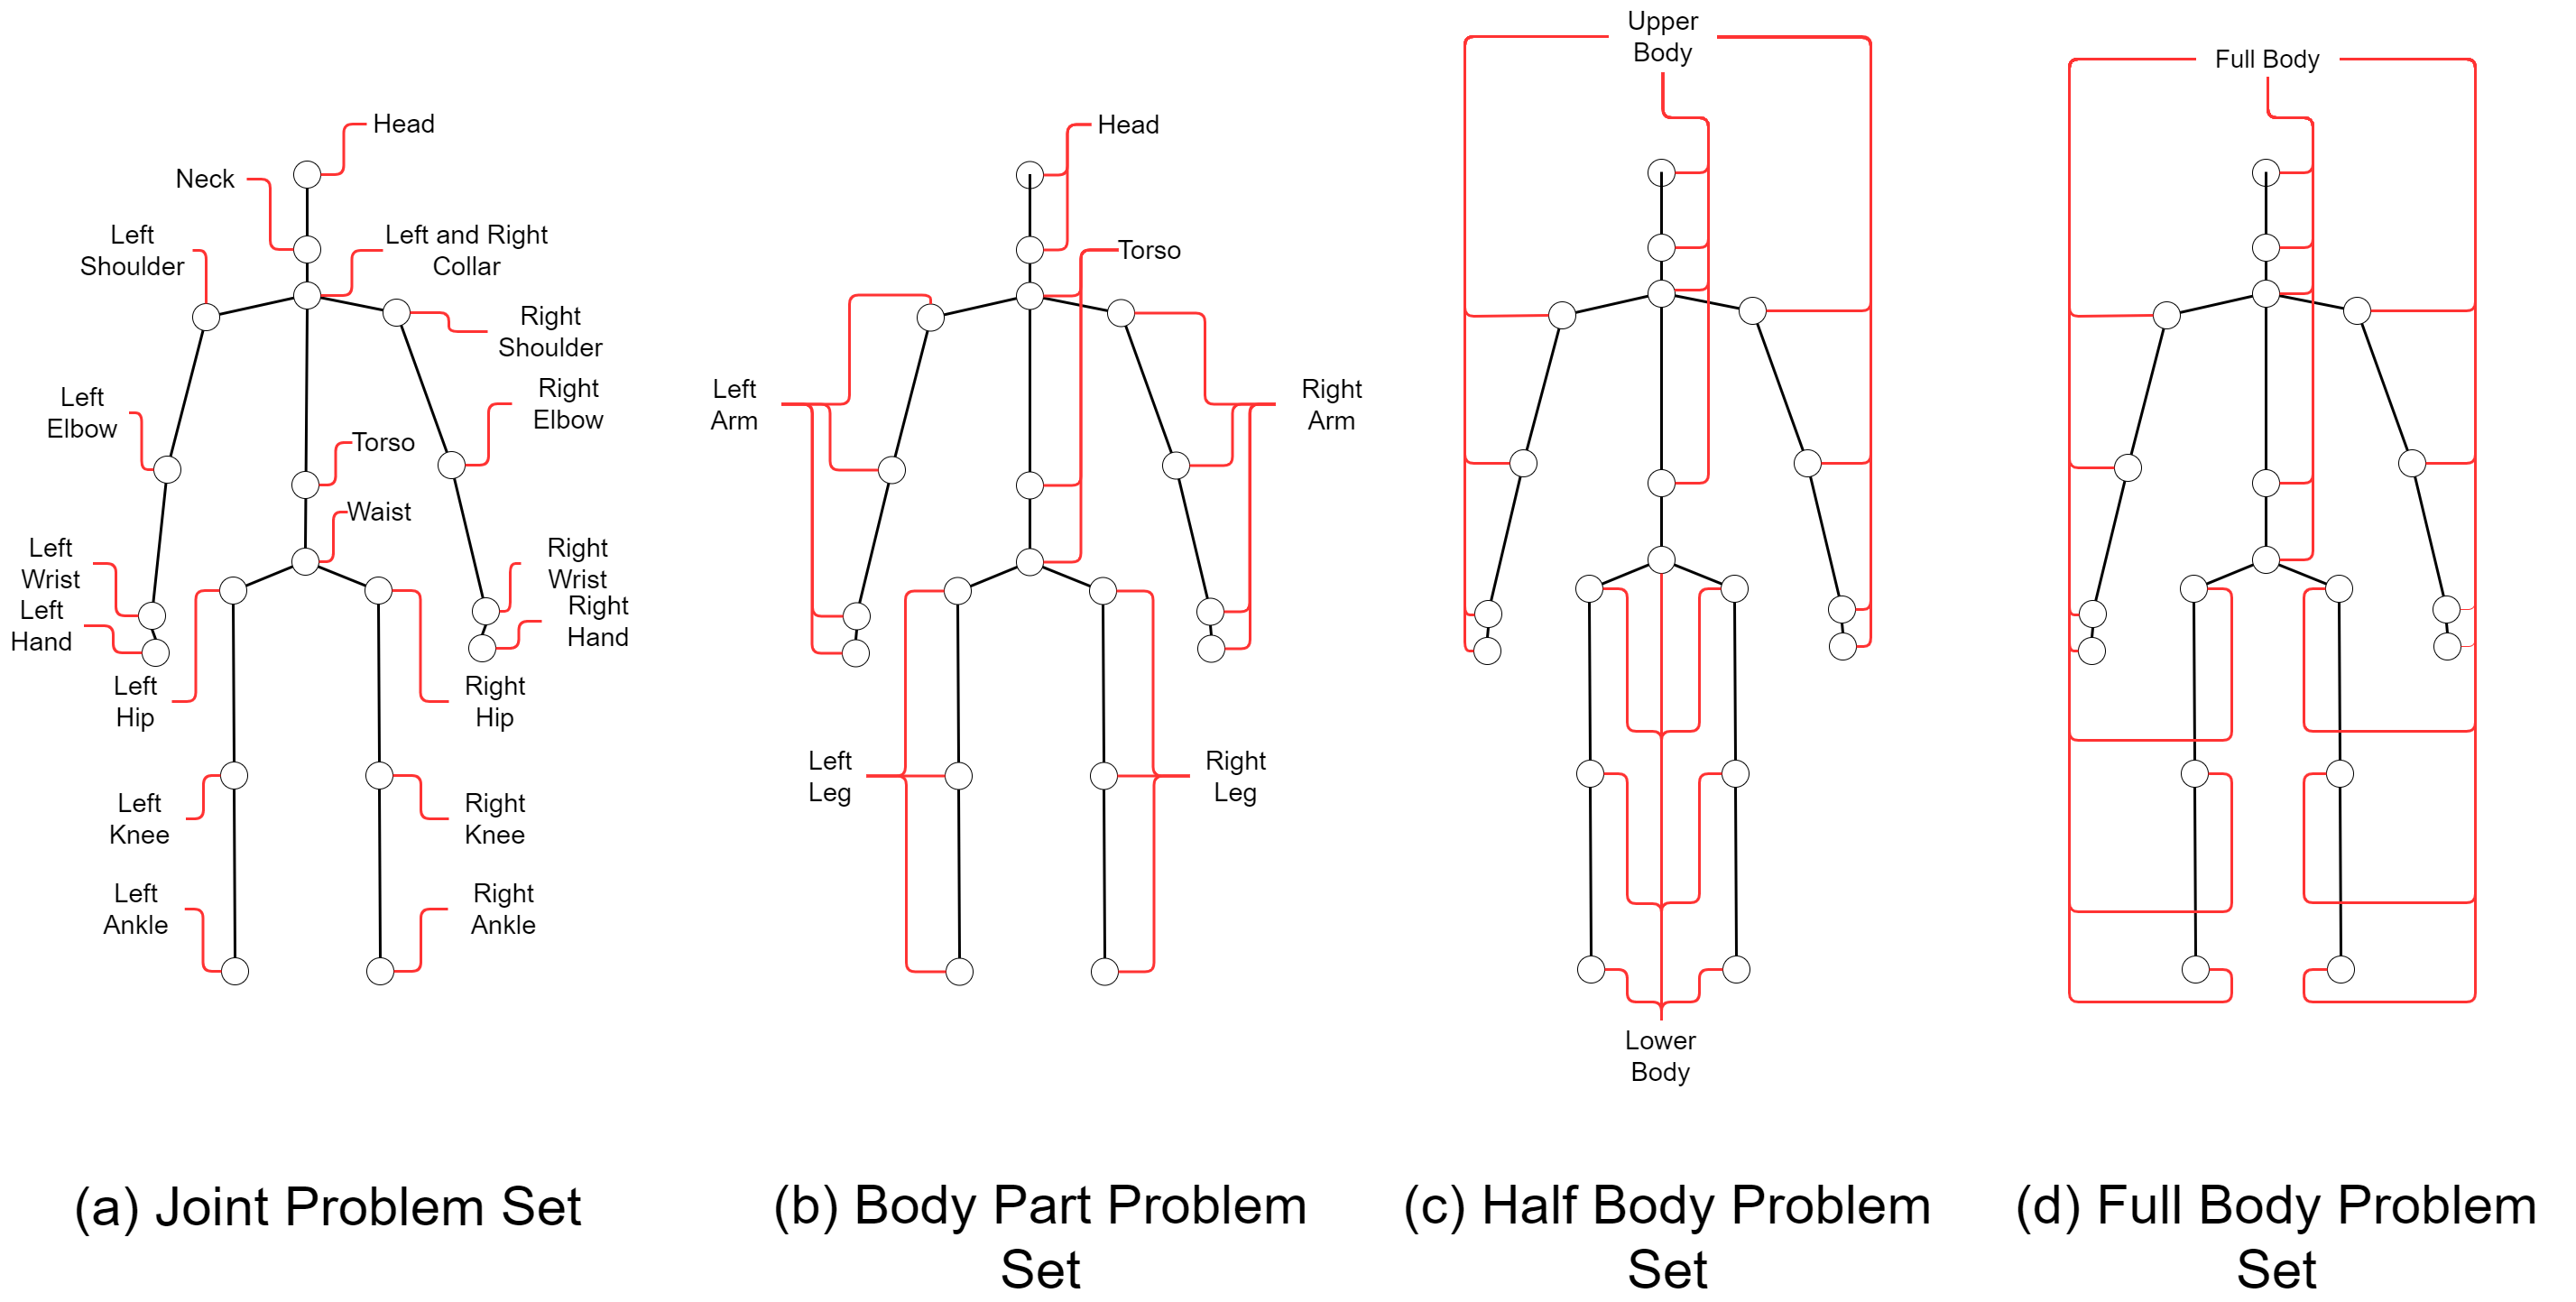
\includegraphics[width=\textwidth]{figures/HPE/problem_sets.png}
  \caption[Visualisation of the Problemsets]{The visualisation of the different problem sets, (a) Joint Problem Set, (b) Body Part Problem Set, (c) Half Body Problem Set, and (d) Full Bod Problem Set.}
  \label{fig:ps}
\end{figure}
